
\documentclass[a4paper,10pt,twoside]{paper}
\usepackage{CJK}
\usepackage{multicol}
\usepackage{graphicx}
\usepackage{subfigure}
\usepackage{booktabs}
\usepackage{amssymb,bm,mathrsfs,bbm,amscd}
\usepackage[tbtags]{amsmath}
\usepackage{lastpage}
\usepackage[justification=centering]{caption}
\usepackage{epstopdf}
\usepackage{diagbox}

\begin{CJK*}{UTF8}{gbsn}

	\begin{document}

	\fancyhead[c]{\small Chinese Physics C~~~Vol. XX, No. X (201X)
	XXXXXX} \fancyfoot[C]{\small 010201-\thepage}
	\footnotetext[0]{Received XX XXXX 20XX}

	\title{The event rate estimation for JUNO experiment \thanks{Supported by National Natural Science Foundation of China (NSFC) under Contracts Nos. xxx, xxx; the Chinese Academy of Sciences (CAS) Large-Scale Scientific Facility Program; Joint Large-Scale Scientific Facility Funds of the NSFC and CAS under Contracts Nos.  U1232201, U1332201.} }


	\author{Fang Xiao(方肖)$^{1,2}$\email{fangx@ihep.ac.cn}
		%      \quad Deng Zi-Yan(邓子艳)$^{2}$
		%     \quad Wen Liang-Jian(温良剑)$^{2}$
		%      \quad Li Wei-Dong(李卫东)$^{2}$\\
		%      \quad Yu Chun-Xu(喻纯旭)$^{1}$
		%      \quad Lin Tao(林韬)$^{2}$
	}
	\maketitle

	\address{
		$^1$ School of Physics, Sichuan University, Chengdu 610065 , China\\
		$^2$ Institute of High Energy Physics, Chinese Academy of Sciences, Beijing 100049, China\\
	}

	\begin{abstract}
		ToDo

	\end{abstract}


	\begin{keyword}
		JUNO,  event rate, computing resource
	\end{keyword}

	\begin{pacs}
		29.40.Mc,29.85.Fj
	\end{pacs}

	\footnotetext[0]{\hspace*{-3mm}\raisebox{0.3ex}{$\scriptstyle\copyright$}2013
		Chinese Physical Society and the Institute of High Energy Physics
		of the Chinese Academy of Sciences and the Institute
	of Modern Physics of the Chinese Academy of Sciences and IOP Publishing Ltd}

	\begin{multicols}{2}

		\section{Introduction}
		JUNO\cite{lab1}(The Jiangmen Underground Neutrino
		Observatory) is a multipurpose neutrino experiment. It is
		designed to determine neutrino mass hierarchy and precisely
		measure oscillation parameters by detecting reactor
		neutrinos from the Yangjiang and Taishan Nuclear Power
		Plants. It also intended to observe supernova neutrinos,
		study the atmospheric, solar neutrinos and geo-neutrinos,
		and perform exotic searches.

		The JUNO experiment hall is located in Kaiping, jiangmen,
		in Southern China. It's about 53 km away from Yangjiang
		and Taishan Nuclear Power Plants, both of which are
		under construction. The planned total thermal power of
		these reactors is 36 GW. In addition, there are no other
		nuclear power plants within 200 km.  The  20-thousand-ton
		liquid scintillator detector of unprecedented 3\% energy
		resolution (at 1 MeV) is installed at 700-meter deep
		underground to suppress backgrounds. 

		The experiment hall is expected to be finished at 2019. 
		It is possible to get data from the experiment at 2020.
	 	The JUNO event rate is very important for JUNO experiment 
		design. So we want to estimate JUNO
		event rate by theory and Geant4 simulation. The
		JUNO event rate is composed of signal rate and background
		rate.With the estimated JUNO event rate,we can estimate the
		offline computing resource such as cpu, disk, which we 
		needed to do offline data saving and analyzing.The estimated
		JUNO event rate can also help the online electronic design.

		In the beginning, for the central detector we proposed
		three design options: acrylic option, balloon option and 
		module option. According to the Geant4 detector simulation,
		the module option was abandoned. Since the acrylic option
		and balloon option are similar, we study the acrylic option
		to estimate JUNO event rate.


		
		%For the backgrounds such as natural radioactivity background(U, Th, K), cosmic muons, the event rate of JUNO is possibly large.  


		\section{JUNO detector scheme}
		The JUNO detector is composed of a central detector, a water
		cherenkov detector and a muon tracker(shown in Fig.1).The 
		central detector is a LS detector of 20kton fiducial mass and
		3\%/$\sqrt{E(MeV)}$ energy resolution.The central detector is
		submerged in a water pool to be shielded from natural 
		radioactivities from the surrounding rock and air.The water pool
		is equipped with PMTs to detect the cherenkov light from muons.
		On top of the water pool, there is a another muon detector to 
		accurately measure the muon track.
		\begin{center}
			%\includegraphics[width=6cm]{acrylicoption.png}
			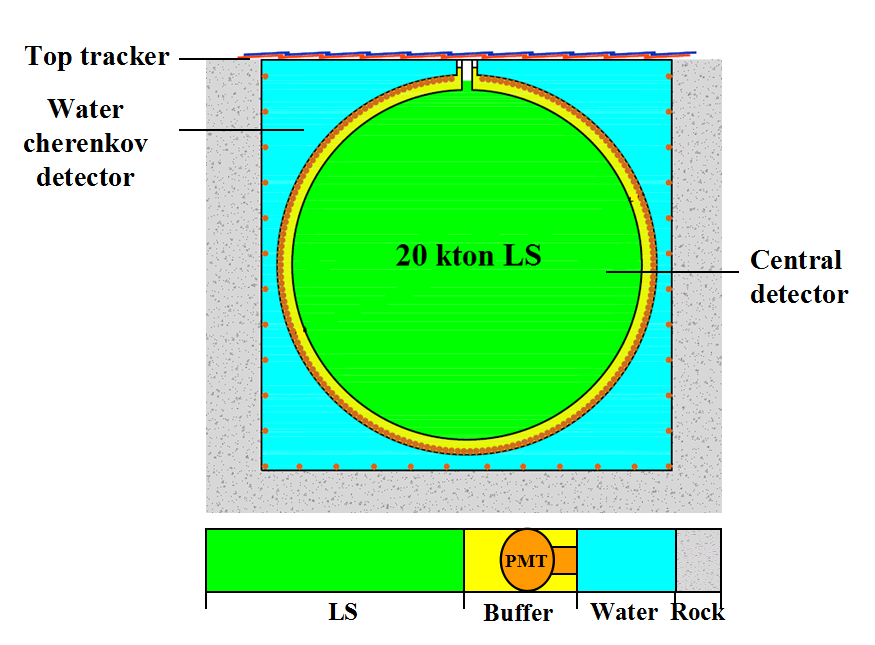
\includegraphics[width=7cm]{CD.png}
			\figcaption{\label{fig2}   Acrylic option }
		\end{center}

		For the central detector, there are two design options at 
		present. The default option is acrylic vessel with stainless
		steel truss. The backup option is liquid balloon with stainless
		steel vessel. Since the two options are similar , we just 
		consider the acrylic option when estimate the event rate.

		In this option, the inner acrylic tank is spherically 
		shaped holding 20 kton LS.The acrylic sphere is supported 
		by the steel truss while the truss is held by some supporting 
		legs at the bottom of the water pool in the experiment hall. 
		The thickness of the acrylic tank is 12 cm. Between the 
		acrylic sphere and the truss, there are many PMTs carried 
		inward facing to the truss to detect the optical signal from LS.
   		Ultrapure water is filled in as shielding liquid outside of the    		
		acrylics tank.	


		\section{The source of event }

		%In JUNO experiment, particles deposit energy in LS and release
		%photons.If the energy of the photons which detected by the PMT
		%exceed the trigger system's energy threshold, the detector will
		%record the electronic output information as a event.

		The event rate we discussed is singles rate that signals from
		particles depositing visible energy greater than trigger 
		system's energy threshold in LS.
		

		Although JUNO is a multi-purpose neutrino experiment.The main 
		physics
		goal is to determine neutrino mass hierarchy and precisely
		measure oscillation parameters by detecting reactor neutrinos 
		from the Yangjiang and Taishan Nuclear Power Plants. So we 
		consider the reactor neutrinos as the main source of signal event.

		
		The reactor electron antineutrino interacts with proton via 
		the inverse $\beta$-decay(IBD) reaction in the liquid 
		scintillator, and releases a positron and a neutron. 
		The positron depositsits energy quickly, providing a prompt 
		signal. The energy of positron carries most of the kinetic 
		energy of the neutrino.
		The neutron is captured by proton after an average time of 
		200$\mu$s, then releases a 2.2 MeV gamma, providing a delayed 
		signal. The coincidence of prompt-delayed signals provides a 
		distinctive antineutrino signature. The estimated IBD reaction 
		rate is about 40/day\cite{lab2}. 
		
		The signals is a small part of event source. The most of
		the event source is background.The background is composed of
		the radioactivity in detector materials and detector 
		surrounding, the cosmic muon and the electronic dark noise.

		The background induced by cosmic ray muon is the main background
		and not easy to remove. Muon can induce high energy neutron as
		fast neutron background. And muon spallation can induce Li9/He8
		background.

		The electronic dark noise is mainly caused by thermal 
		emission of electrons and radioactivity from components of the 
		PMTs. Although the energy of dark noise is small, it may exceed
		the energy threshold when the energy threshold is low.


		\section{The event rate estimation of central detector}
		The JUNO detector consists of a central detector, a water 
		cherenkov detector and a muon tracker.So we estimate the event
		rate of each part respectively.The central detector is the 
		main part of JUNO detector.As we mentioned previously, 
		the signal
		rate is about 40/day. We will discuss the background in the 
		following.

		\subsection{Natural radioactivity estimation}
		Natural radioactivity exists in the materials of central 
		detector.
		The materials of central detector in the acrylic option mainly
		include LS, acrylic, oxygen-free copper, stainless steel, as
		well as the glass of PMT.
		The formations of these materials in different conditions 
		cause more or less existence of radioelement.
		The Rn in the water pool also induced radioactivity.
		The singles rate of each material's natural radioactivity 
		in different energy threshold is 
		listed in table.1. The detailed discussion can be found in
		the reference\cite{lab3}.

	\end{multicols}
	\begin{center}
		\tabcaption{ \label{tab1}  The inner singles rates}
		\footnotesize
		\begin{tabular*}{170mm}{@{\extracolsep{\fill}} c c c c c c c c}
			\toprule  Singles Rate(Hz)&LS &Glass &Acrylic  &Steel &Copper &Rn &Sum \\
			\hline
			E$>$0.7MeV &2.39   &2.43  &69.23  &0.89  &0.82 &17.31   &93.07  \\
			E$>$0.6MeV &4.26   &2.66  &75.26  &0.95  &0.94 &19.79   &103.86 \\
			E$>$0.5MeV &12.06  &2.83  &81.49  &0.98  &1.06 &23.36   &121.78 \\
			E$>$0.4MeV &13.86  &3.24  &87.84  &1.22  &1.29 &26.11   &133.56 \\
			E$>$0.3MeV &15.51  &3.72  &98.57  &1.57  &1.51 &31.60   &152.48 \\
			E$>$0.2MeV &17.16  &4.12  &117.33 &1.80  &1.89 &39.85   &182.15 \\
			E$>$0.1MeV &352.36 &5.27  &149.26 &2.22  &2.60 &54.97   &566.68 \\
			\bottomrule
		\end{tabular*}
	\end{center}
	\begin{multicols}{2}


		\subsection{Muon estimation}
		In order to reduce muon background, the central detector is 
		located in 460 meters underground level. There are about 700
		meters rock on the top of the experiment hall.Muno rate is about
		0.003Hz/$m^2$ and average muon energy is 214GeV from simulation
		study\cite{lab4}. Compared to the ground surface, the muon flux
		is reduced about 60000times.

		The radius of LS sphere is 17.7m, so the muon rate in central
		detector is about: $\pi \times 17.7^2 \times 0.003 = 2.95$Hz.

		Cosmic muon rays can also produce a large number of neutrons
		in the rock around central,these neutron can produce fast 
		neutron background in the central detector. If water shield
		thickness is 2.5 meters in JUNO, fast neutron ratio is 0.3\%,
		considering detector volume and geometry effects.

		Spallation muon interact with scintillator can induce Li9/He8
		background. We use the  formula to estimate Li9/He8 
		background: $Y_n = C \times Q_c \times E^\alpha$.

		In this formula we assume the yield is power law function of 
		muon energy. $Q_c$ is carbon density factor for different
		liquid scintillator.

		In JUNO experiment the mean muon energy is 215GeV, the mass of
		liquid scintillator is 20kton, the muon flux is 0.003Hz/$m^2$, 
		the $\alpha$ in formula is 1.06$\pm$0.2 .The yield of 
		Li9/He8 is $(2.3\pm0.5\times10^{-7})(\mu g /cm^2)^{-1}$.
		So the Li9/He8 event rate in JUNO is $57\pm14$/day.




		\subsection{Dark noise estimation}

		To estimate the event rate of dark noise, we suppose a detector
		has N PMTs, each PMT has dark current rate f Hz, multiplicity 
		trigger threshold is m PMTs, trigger integration time is $\tau$
		ns. So the noise rate can be calculated by the below formula:

		\begin{displaymath}
			R = \frac{1}{\tau}\sum_{i=m}^{N}iC^{i}_{N}(f\tau)^i
			(1-f\tau)^{N-i}
		\end{displaymath}


		In JUNO experiment, we assume the total PMT number is 17746, 
		the dark current rate of each PMT is 50kHz, the trigger 
		integration time is 300ns. The number of photons which are
		received by PMTs is 1200, when the visible energy is 1MeV.
		So the estimated dark noise event rate can be shown in Fig2.

		\begin{center}
			%\includegraphics[width=6cm]{acrylicoption.png}
			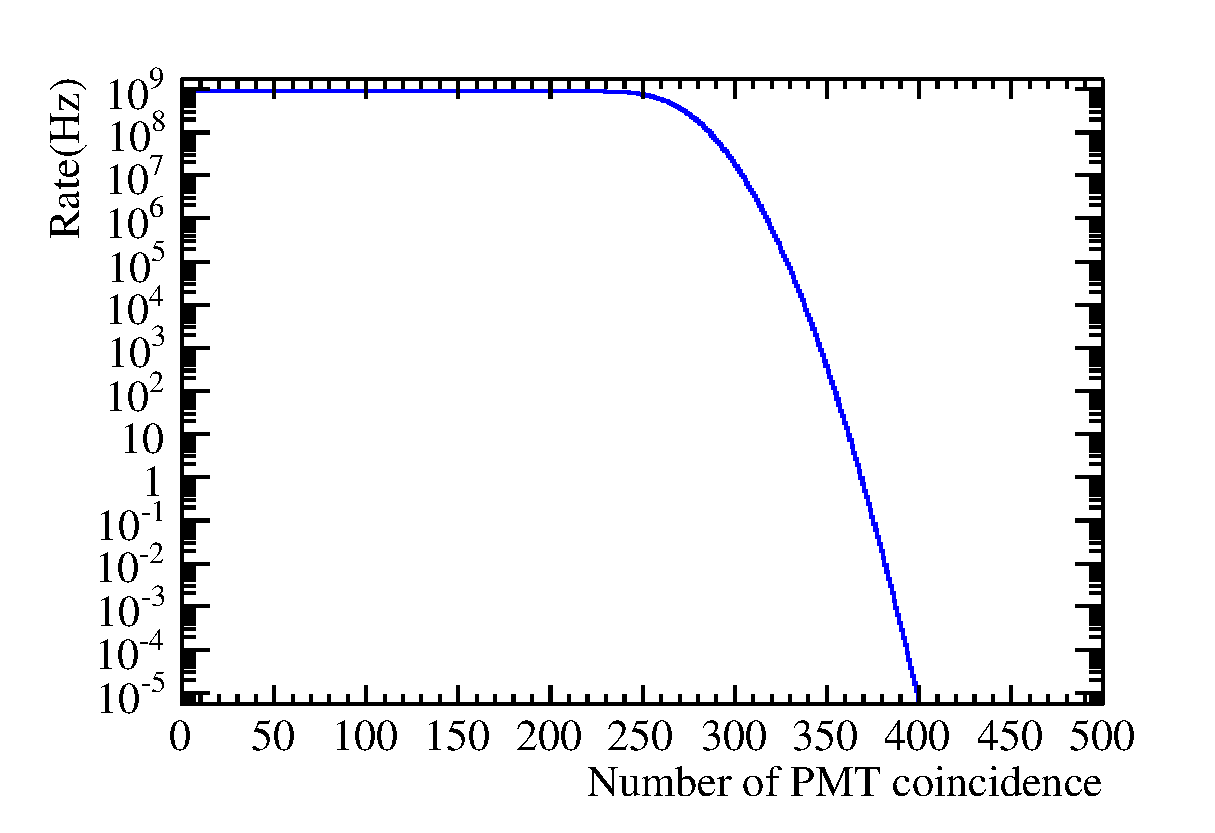
\includegraphics[width=8cm,height=6cm]{Noise_rate_50kHz_300ns.eps}
			\figcaption{\label{fig2}    
				Dark noise event rate when trigger integration time is 300ns 
			}
		\end{center}


		From Fig2 we can see the energy threshold must greater than 0.3MeV. So that
		the dark noise will induce few background event rate. 


		\subsection{A promising secondary trigger system design}

		If we just study the IBD event, we can set the first trigger system's energy
		threshold to 0.7MeV. So the dark noise will induce few event rate, and from 
		Table.1 we can see the total radioactivity background event rate in central
		detector is 75.75Hz ,when energy threshold greater than 0.7 MeV.

		But if we want study solar neutrinos, supernova neutrinos and other low energy neutrino sources,
		, low energy threshold is very important. When the energy threshold is decreased,
		the background rate of radioactivity and dark noise will be increased. 
		So we proposed a new secondary trigger system design to reduce the background rate.
		
		We can reduce radioactivity background by the vertex of event, because the  radioactivity 
		from  acrylic tank, oxygen-free copper and stainless steel most deposit energy at the edge of
		LS sphere. Vertex reconstruction algorithm in FPGA is difficult and need too much resource.
		So we can't reconstruct event vertex accurately online. But we can use another method to find
		the approximate event vertex.

		In this method, we want to correct the PMT's first
		hit time by deducting photon's flying time in LS. 
		Because the distribution of PMT's corrected first hit time
		is narrow, we can use this character to find the approximate event vertex. 
		If we know the vertex of the event, we can know the photon's flying time from vertex to each
		PMT.
		So it is easy to correct the PMT's first hit time
		by deducting TOF(Time Of Fly).

		But as mentioned before , it is difficult to find event
		vertex accurately by FPGA's algorithm online. So we
		divide the central detector volume into 179 5m$\times$5m$\times$5m
		cubic regions. We assume each region's center as a possible event vertex.
		For each event, we correct the PMT's 
		first hit time for each possible event vertex in parallel.


		As we have 179 cubic regions, we can get 179 distributions of corrected 
		PMT's first hit time. 
		If the region contain the true event vertex, 
		the distribution of corrected PMT's first hit time 
		will be most narrow.
		So we can find the region which contain the event vertex. 
		And then using the center of the region as the approximate
		event vertex.

		To demonstrate this method is viable, we simulated 4MeV 
		positron generated at R=15m in central detector. 
		Fig.3 show the PMT's first hit time without TOF corrected.
		Fig.4 show the PMT's first hit time with TOF corrected.


		\begin{center}
			%\includegraphics[width=6cm]{acrylicoption.png}
			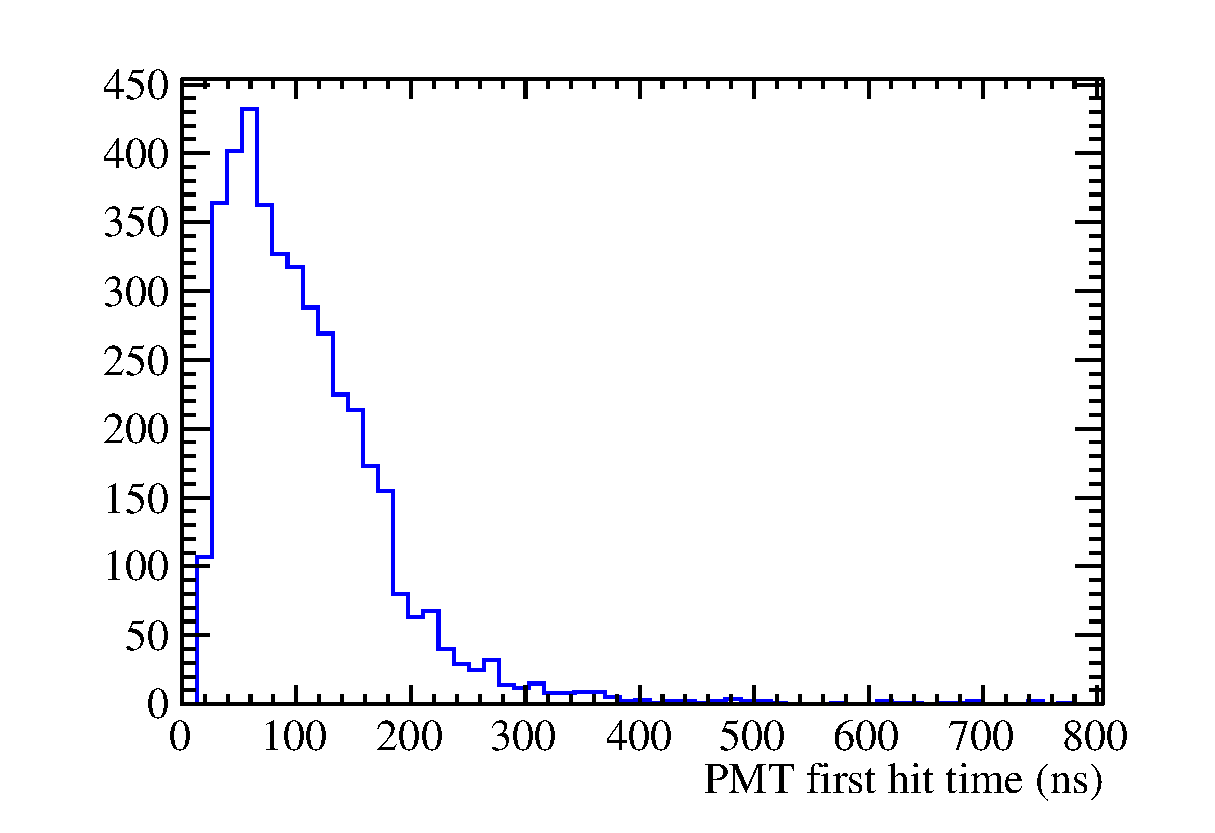
\includegraphics[width=8cm,height=6cm]{4MeV_e+_PMT_first_hitTime.eps}
			\figcaption{\label{fig2}   PMT's first hit time without TOF corrected 
			}
		\end{center}


		\begin{center}
			%\includegraphics[width=6cm]{acrylicoption.png}
			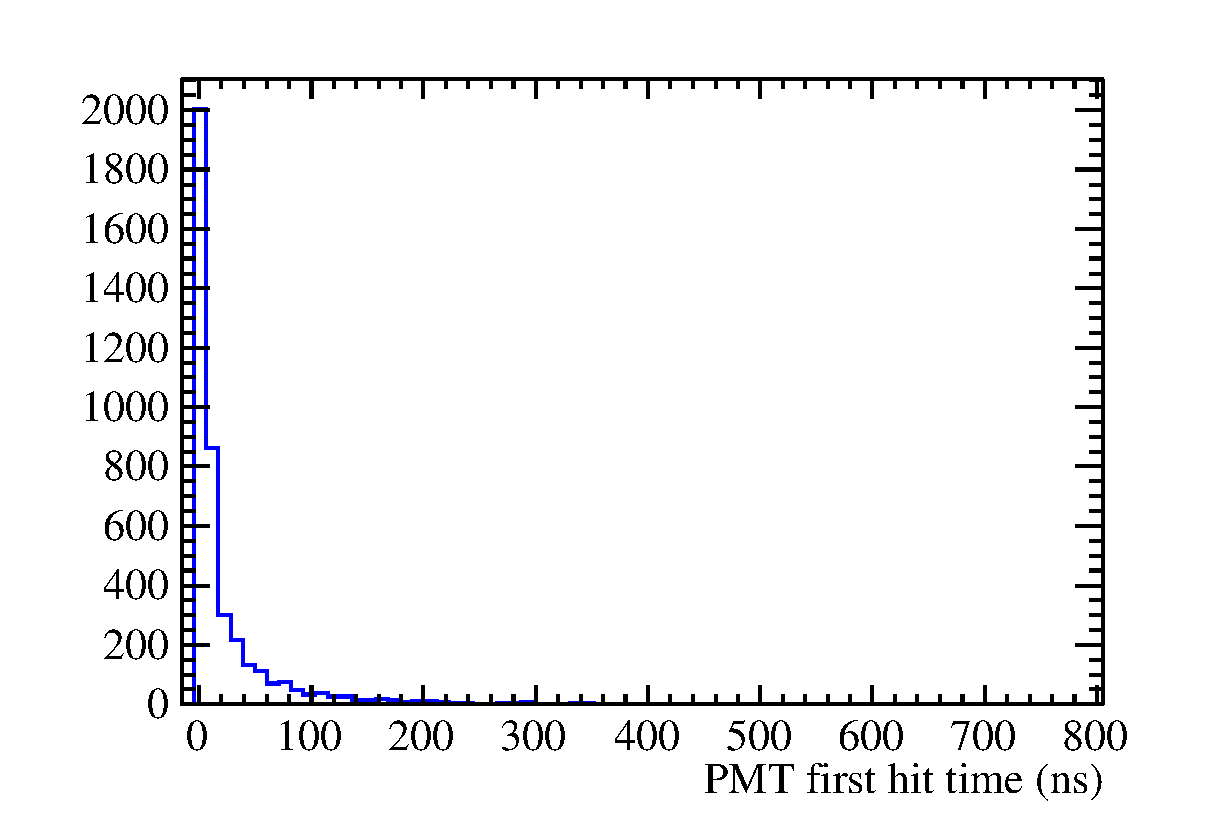
\includegraphics[width=8cm,height=6cm]{4MeV_e+_PMT_first_hitTime_corrected.eps}
			\figcaption{\label{fig2}   PMT's first hit time with TOF corrected 
			}
		\end{center}


		From Fig.3 and Fig.4 we can see the distribution of PMT's first hit time is narrow
		when we do the TOF correction. So the width of distribution can be used to check if 
		the TOF correction is valid.


		With the reconstructed approximate vertex, we can
		set different radius threshold to reduce radioactivity
		backgrounds. In the trigger system, the first and secondary trigger system are in parallel. 
		In the first trigger system, we record the events which the visible energy
		greater than energy threshold. In the secondary trigger system, 
		we record the events which the visible energy less than energy threshold 
		and the reconstructed vertex position less than radius threshold.
		In table.2 we show the central detector's sum radioactivity background rate
		on different energy and radius threshold.


	\end{multicols}
	\begin{center}
		\tabcaption{ \label{tab1} The sum radioactivity singles rates in central detector on different energy and radius threshold }
		\footnotesize
		\begin{tabular*}{170mm}{@{\extracolsep{\fill}} c c c c c c c}
			\toprule  Sum Radioactivity Single Rate(Hz)&E$>$0.1MeV & E$>$0.2MeV & E$>$0.3MeV & E$>$0.4MeV & E$>$0.5MeV & E$>$0.6MeV \\
			\hline
			R$<$10m &142.368  &98.332  &96.9047 &95.9515 &95.2811  &93.7126 \\
			R$<$11m &153.808  &99.1398 &97.5285 &96.4432 &95.6678  &93.8127 \\
			R$<$12m &199.79   &102.354 &100.039 &98.4438 &97.2644  &94.2101 \\
			R$<$13m &249.897  &105.33  &102.395 &100.341 &98.7855  &94.5798 \\
			R$<$14m &249.897  &105.33  &102.395 &100.341 &98.7855  &94.5798 \\
			R$<$15m &289.921  &112.385 &107.156 &103.627 &101.128  &95.4422 \\
			R$<$16m &458.269  &148.923 &131.168 &119.73  &112.381  &99.866  \\
			R$<$17m &540.865  &173.071 &146.688 &129.847 &119.277  &102.776 \\
			\bottomrule
		\end{tabular*}
	\end{center}
	\begin{multicols}{2}


		The promising secondary trigger system not only can
		reduce radioactivity background event rate, but also can
		reduce dark noise event rate.


		In Fig.2 we can see if we set energy threshold below
		0.3MeV, the dark noise event rate will be high. But in
		Fig.4 we can see the width of PMT's first hit time distribution
		is narrow when we do the TOF correction.
		If we find the approximate vertex of
		event, we can correct the PMT's first hitTime. And the
		width of PMT's first hit time distribution will be narrow.
		So we can reduce the trigger integration time from 300ns
		to 50ns. And then we can use the formula (1) to estimate
		the dark noise event rate, when trigger integration time
		is 50ns. The rescult is shown in Fig.5.


		\begin{center}
			%\includegraphics[width=6cm]{acrylicoption.png}
			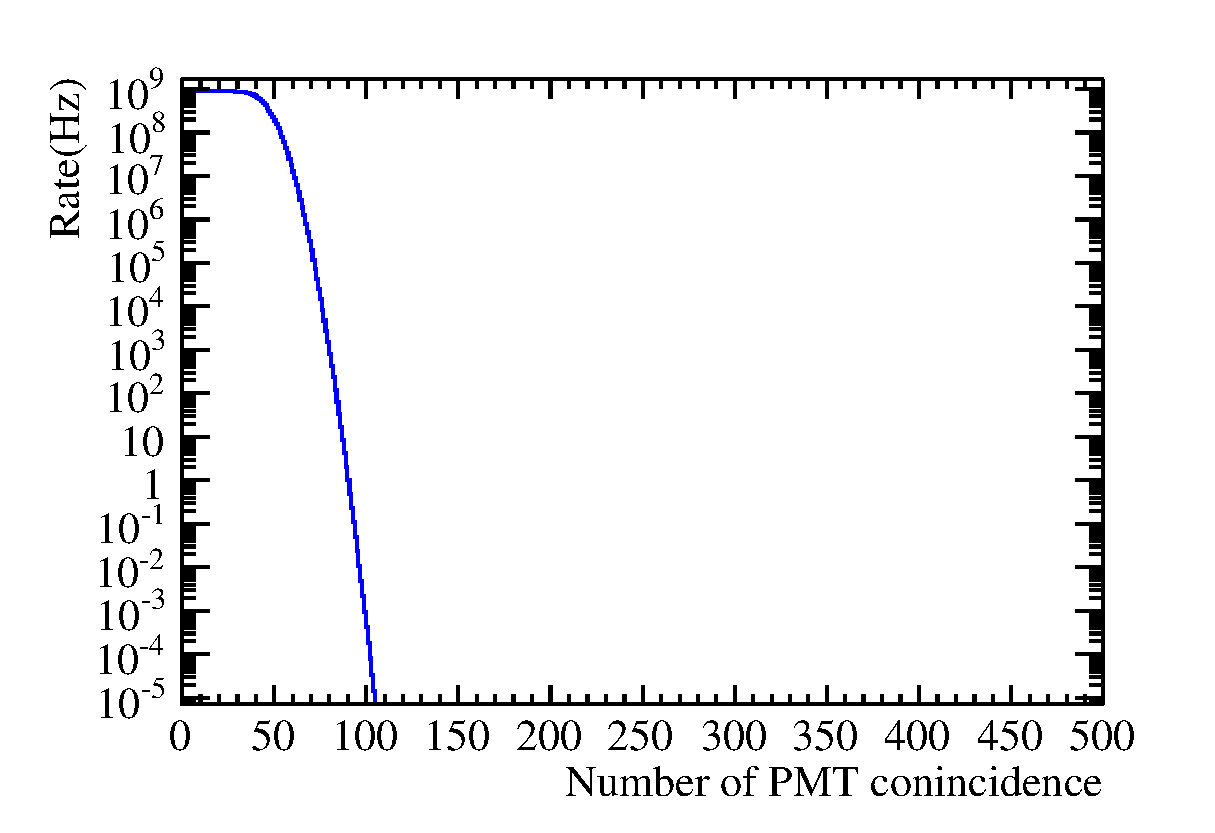
\includegraphics[width=8cm,height=6cm]{Noise_rate_50kHz_50ns.eps}
			\figcaption{\label{fig2}    
				Dark noise event rate when trigger integration time is 50ns 
			}
		\end{center}



		\section{The event rate estimation of water pool}

		\section{The event rate estimation of top tracker}

		\vspace{-1mm}
		\centerline{\rule{80mm}{0.1pt}}
		\vspace{2mm}

		\begin{thebibliography}{90}

				\vspace{3mm}


			\bibitem{lab1}Y.F. Li, J. Cao, Y.F. Wang and L. Zhan, Unambiguous Determination of the Neutrino Mass Hierarchy Using Reactor Neutrinos Phys. Rev. D 88, 013008 (2013).
			\bibitem{lab2}Y.F. Li, J. Cao, Y.F. Wang and L. Zhan, Unambiguous Determination of the Neutrino Mass Hierarchy Using Reactor Neutrinos Phys. Rev. D 88, 013008 (2013).
			\bibitem{lab3}Y.F. Li, J. Cao, Y.F. Wang and L. Zhan, Unambiguous Determination of the Neutrino Mass Hierarchy Using Reactor Neutrinos Phys. Rev. D 88, 013008 (2013).

		\end{thebibliography}

	\end{multicols}

	%\clearpage
\end{CJK*}
\end{document}
